
A Janus dendrimer is a amphiphilic dendrimer in which the hydrophobic part is concentrated in a side while the hydrophilic part is concentrated in the opposite side.
We illustrated this kind of molecule by concentrating the PAMAM BBs in one region and the PPI BBs at the opposite region of the resulting dendrimer, as depicted in Figure \ref{fig:JanusG1}.
This way, the resulting dendrimer is not amphiphilic due to the similar nature of the PAMAM and PPI chemistry, yet it is a Janus-like dendrimer since it is split into two dendrimeric parts.
At the present approach, we used only the dendrimer module for building a method inspired by the divergent synthesis method for creating Janus-like dendrimers.
We illustrate this method by using PAMAM and PPI dendrimers BBs.

\begin{figure}
    \centering
    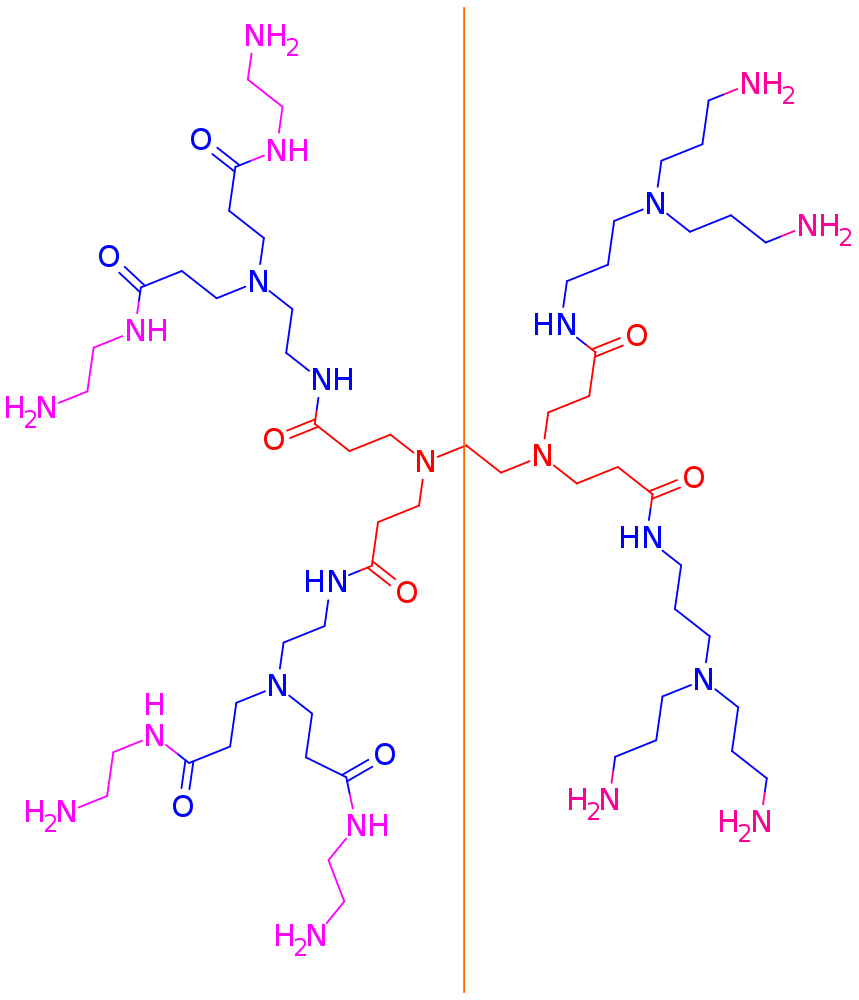
\includegraphics[width=0.5\textwidth]{PAMAM_PPI-Janus/JANUSG1.png}
    \caption{PAMAM/PPI Janus G1 dendrimer.}
    \label{fig:JanusG1}
\end{figure}

The dendrimer module was designed for building homogeneous perfect dendrimers.
Hence, it is not straightforward to build a dendrimer using BBs of different types.
The BBs that are going to be used in this tutorial are exactly the same ones used in previous tutorials (see Figure \ref{fig:JanusBBs}).
These files are provided in the demo directory in pypolybuilder root, whose structure is illustrated below:
\begin{lstlisting}
<path/to/pypolybuilder>/demo/gromacs_format/dendrimer/PAMAM_PPI
\end{lstlisting}
\dirtree{%
.1 PAMAM\_PPI.
.2 core\_PAMAM.itp.
.2 inter\_PAMAM.itp.
.2 ter\_PAMAM.itp.
.2 inter\_PPI.itp.
.2 ter\_PPI.itp.
.2 list\_param.itp.
.2 run.
.3 PAMAM\_PPI.sh.
.3 PAMAM\_PPI.top.
.3 mdp.
}

\begin{figure}
    \centering
    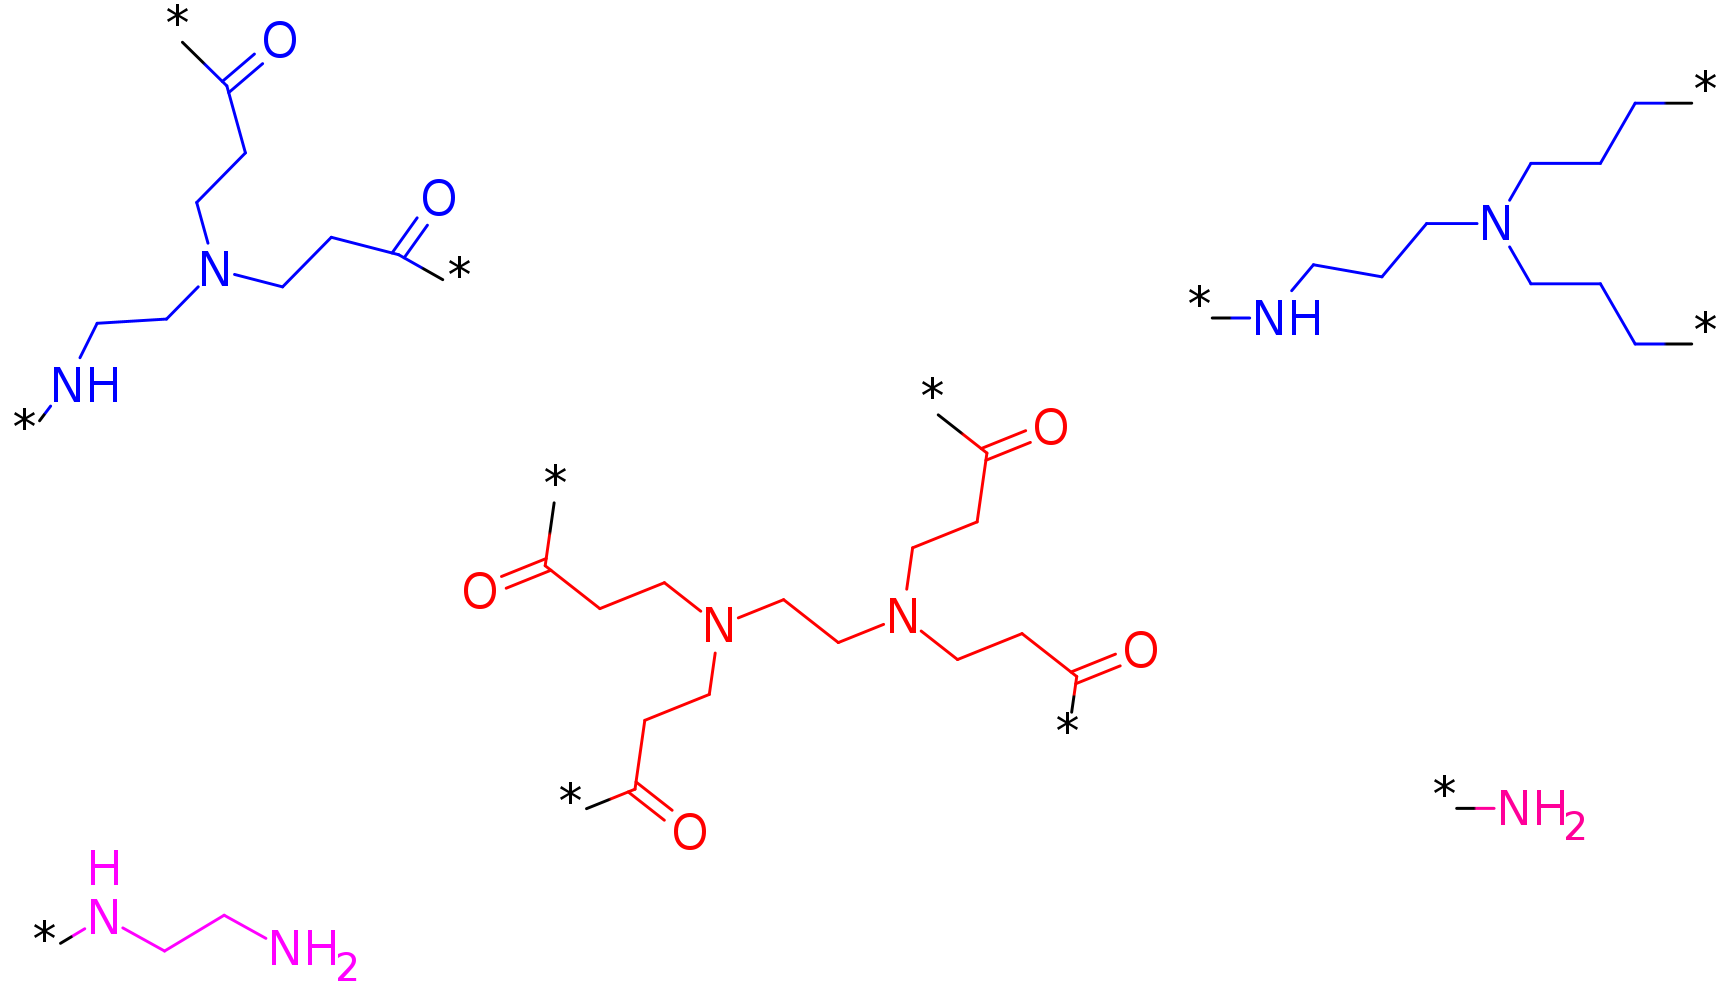
\includegraphics[width=\textwidth]{PAMAM_PPI-Janus/JANUSBBs.png}
    \caption{PAMAM/PPI Janus dendrimer BBs. The PAMAM core block is illustrated in red, intermediary and core blocks are placed on the left in blue and red, respectively. On the right, the BBs for PPI intermediary and core, also in blue and red, respectively.}
    \label{fig:JanusBBs}
\end{figure}

In order to build a Janus dendrimer, we need to make it in two steps.
The whole process is automated in \texttt{how\_to\_run\_this\_example.txt}.
Therefore, this file may be executed with bash in order to get the final geometry.
Nevertheless, the process is described in the following.
First, we need to grow one half of the dendrimer without growing the opposite half.
Afterwards, we use the pyPolyBuilder to grow the second half.
The pyPolyBuilder connects the branches using the dendrimer module according to the \texttt{[ branches ]} field.
The atom indexes in the ``acceptor'' column will receive a new bond from the atom in the ``donor'' column in the incoming new intermediary block.
Therefore, we can edit this field in order to select which branches will be created in each step.
The \texttt{core\_PAMAM.itp} file in this tutorial has its \texttt{[ branches ]} field edited as shown below:

\begin{lstlisting}
[ branches ]
;  donor   acceptor
;   0     10
;   0     13
    0     16
    0     19
\end{lstlisting}

Lines that begin with ``;'' are comments and will not be interpreted by pyPolyBuilder.
With this \texttt{[ branches ]}, the intermediary blocks will only be connected at atoms 16 and 19, respectively.
First, the PAMAM branches are included by using the command line code:

\begin{lstlisting}
python3 ../../../../__main__.py \
--core=core_PAMAM.itp \
--inter=inter_PAMAM.itp \
--ter=ter_PAMAM.itp \
--params=list_param.itp \
--ngen=1 \
--name=PAMH \
--output=PAMAMhalf.itp \
--nogeom \
--dendrimer
\end{lstlisting}

In this command line, \texttt{--core}, \texttt{--inter} and \texttt{--ter} were used for selecting the building blocks, \texttt{--params} for parsing force fields parameter files, \texttt{--ngen} to select the generation of the PAMAM that will be grown, \texttt{--name} for naming the topology, and \texttt{--output} for naming the generated MTF.
Notice that the option \texttt{--gro} was not used here since the geometry will not be optimized and an initial guess for the geometry will not be produced.
Accordingly, we use the \texttt{--nogeom} flag.
As this is just an intermediary step in the process of creating the molecule, only the MTF is needed.
See the Section \ref{sec:CommandLine}.
After the build is done, a new \texttt{PAMAMhalf.itp} MTF with the PAMAM half of the Janus dendrimer (Figure \ref{fig:JanusPAMAMhalf}) will be produced.

\begin{figure}
    \centering
    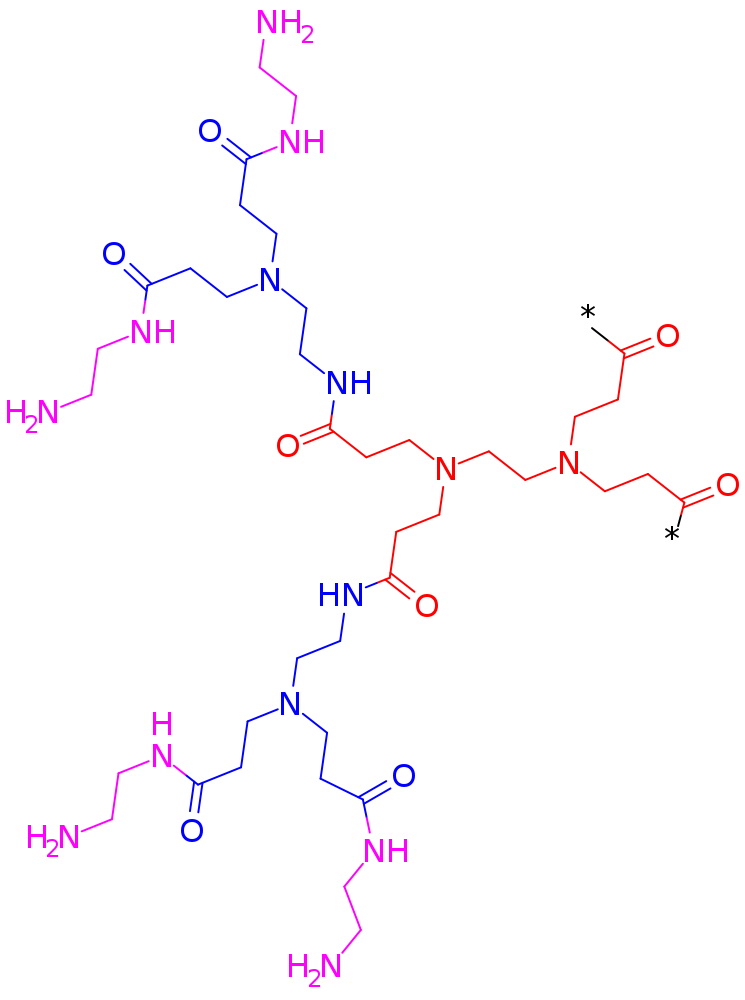
\includegraphics[width=0.4\textwidth]{PAMAM_PPI-Janus/JANUSPAMAMhalf.png}
    \caption{The dendrimer with only the PAMAM BBs attached to the core BB.}
    \label{fig:JanusPAMAMhalf}
\end{figure}

The PAMAM core has 4 branch points, at the atoms 10, 13, 16 and 19.
We have already used the branch points 16 and 19 for growing the part in which we used the PAMAM BBS.
However, the atoms 10 and 13 are available for growing the second half of the dendrimer using the PPI BBs.
We need to edit the \texttt{PAMAMhalf.itp} file
to include the desired \texttt{[ branches ]} shown below in the final of the file:

\begin{lstlisting}
[ branches ]
;  donor   acceptor
    0     10
    0     13
;   0     16
;   0     19
\end{lstlisting}

After editing the \texttt{PAMAMhalf.itp} file, the second part of the dendrimer may be grown by running the following command line:

\begin{lstlisting}
python3 ../../../../__main__.py \
--core=PAMAMhalf.itp \
--inter=inter_PPI.itp \
--ter=ter_PPI.itp \
--params=list_param.itp \
--ngen=1 \
--name=PAMPPI \
--output=PAMAM_PPI.itp \
--gro=PAMAM_PPI.gro \
--dendrimer
\end{lstlisting}

Here, as the geometry is wanted, the \texttt{--nogeom} flag was not used.
Instead, \texttt{--gro} option was used to name the gro file that will be generated.

After pyPolyBuilder has finished the optimization step, one can use any visualization software to check the output geometry. 
Note that the coordinates are generated considering the molecule in vaccum.
Hence, it may not be the expected conformation in solvent (Figure \ref{fig:JanusPPB}).
Because of that, the run directory has some scripts to run a short MD simulation in order to equilibrate the molecule in water using gromacs.
However, these scripts were developed for a specific architecture and needs to be adapted by the user.

\begin{figure}
    \centering
    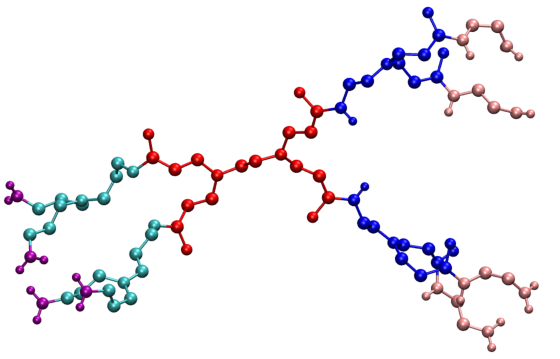
\includegraphics[width=0.5\textwidth]{PAMAM_PPI-Janus/PAMAM_PPI.pdf}
    \caption{The Janus-like dendrimer generated by pyPolyBuilder using PAMAM and PPI BBs. The PAMAM core is displayed in red, PAMAM and PPI intermediaries are displayed, respectively, in blue and cyan, and the terminal PAMAM and PPI blocks are in pink and purple, respectively.
    For instance, in this snapshot, the PAMAM half is at the right side of the structure, and PPI half at the left side.}
    \label{fig:JanusPPB}
\end{figure}

Using the topology generated by pyPolyBuilder, the Janus-like dendrimer was solvated, its energy was minimized, and equilibrations in nvt and npt ensembles were carried out for 100 ps each (Figure \ref{fig:JanusSOL}).

\begin{figure}
    \centering
    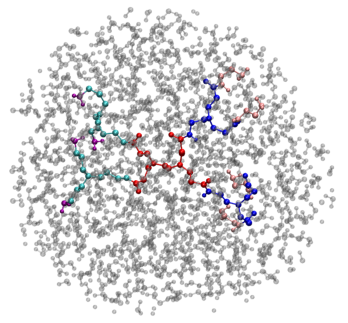
\includegraphics[width=0.5\textwidth]{PAMAM_PPI-Janus/PAMAM_PPISOL.pdf}
    \caption{The created Janus-like structure after equilibration in water solvent.
    Similarly to the Figure \ref{fig:JanusPPB}, PAMAM monomers are at the right side of the molecule while PPI monomers are at the left side, at this snapshot.
    The color scheme was chosen to be the same as in Figure \ref{fig:JanusPPB}.}
    \label{fig:JanusSOL}
\end{figure}
